\documentclass[main.tex]{subfiles}

\begin{document}

\section{Les solutions matérielles}

\subsection{Raspberry Pi}

\begin{figure}[H]
	\centering
	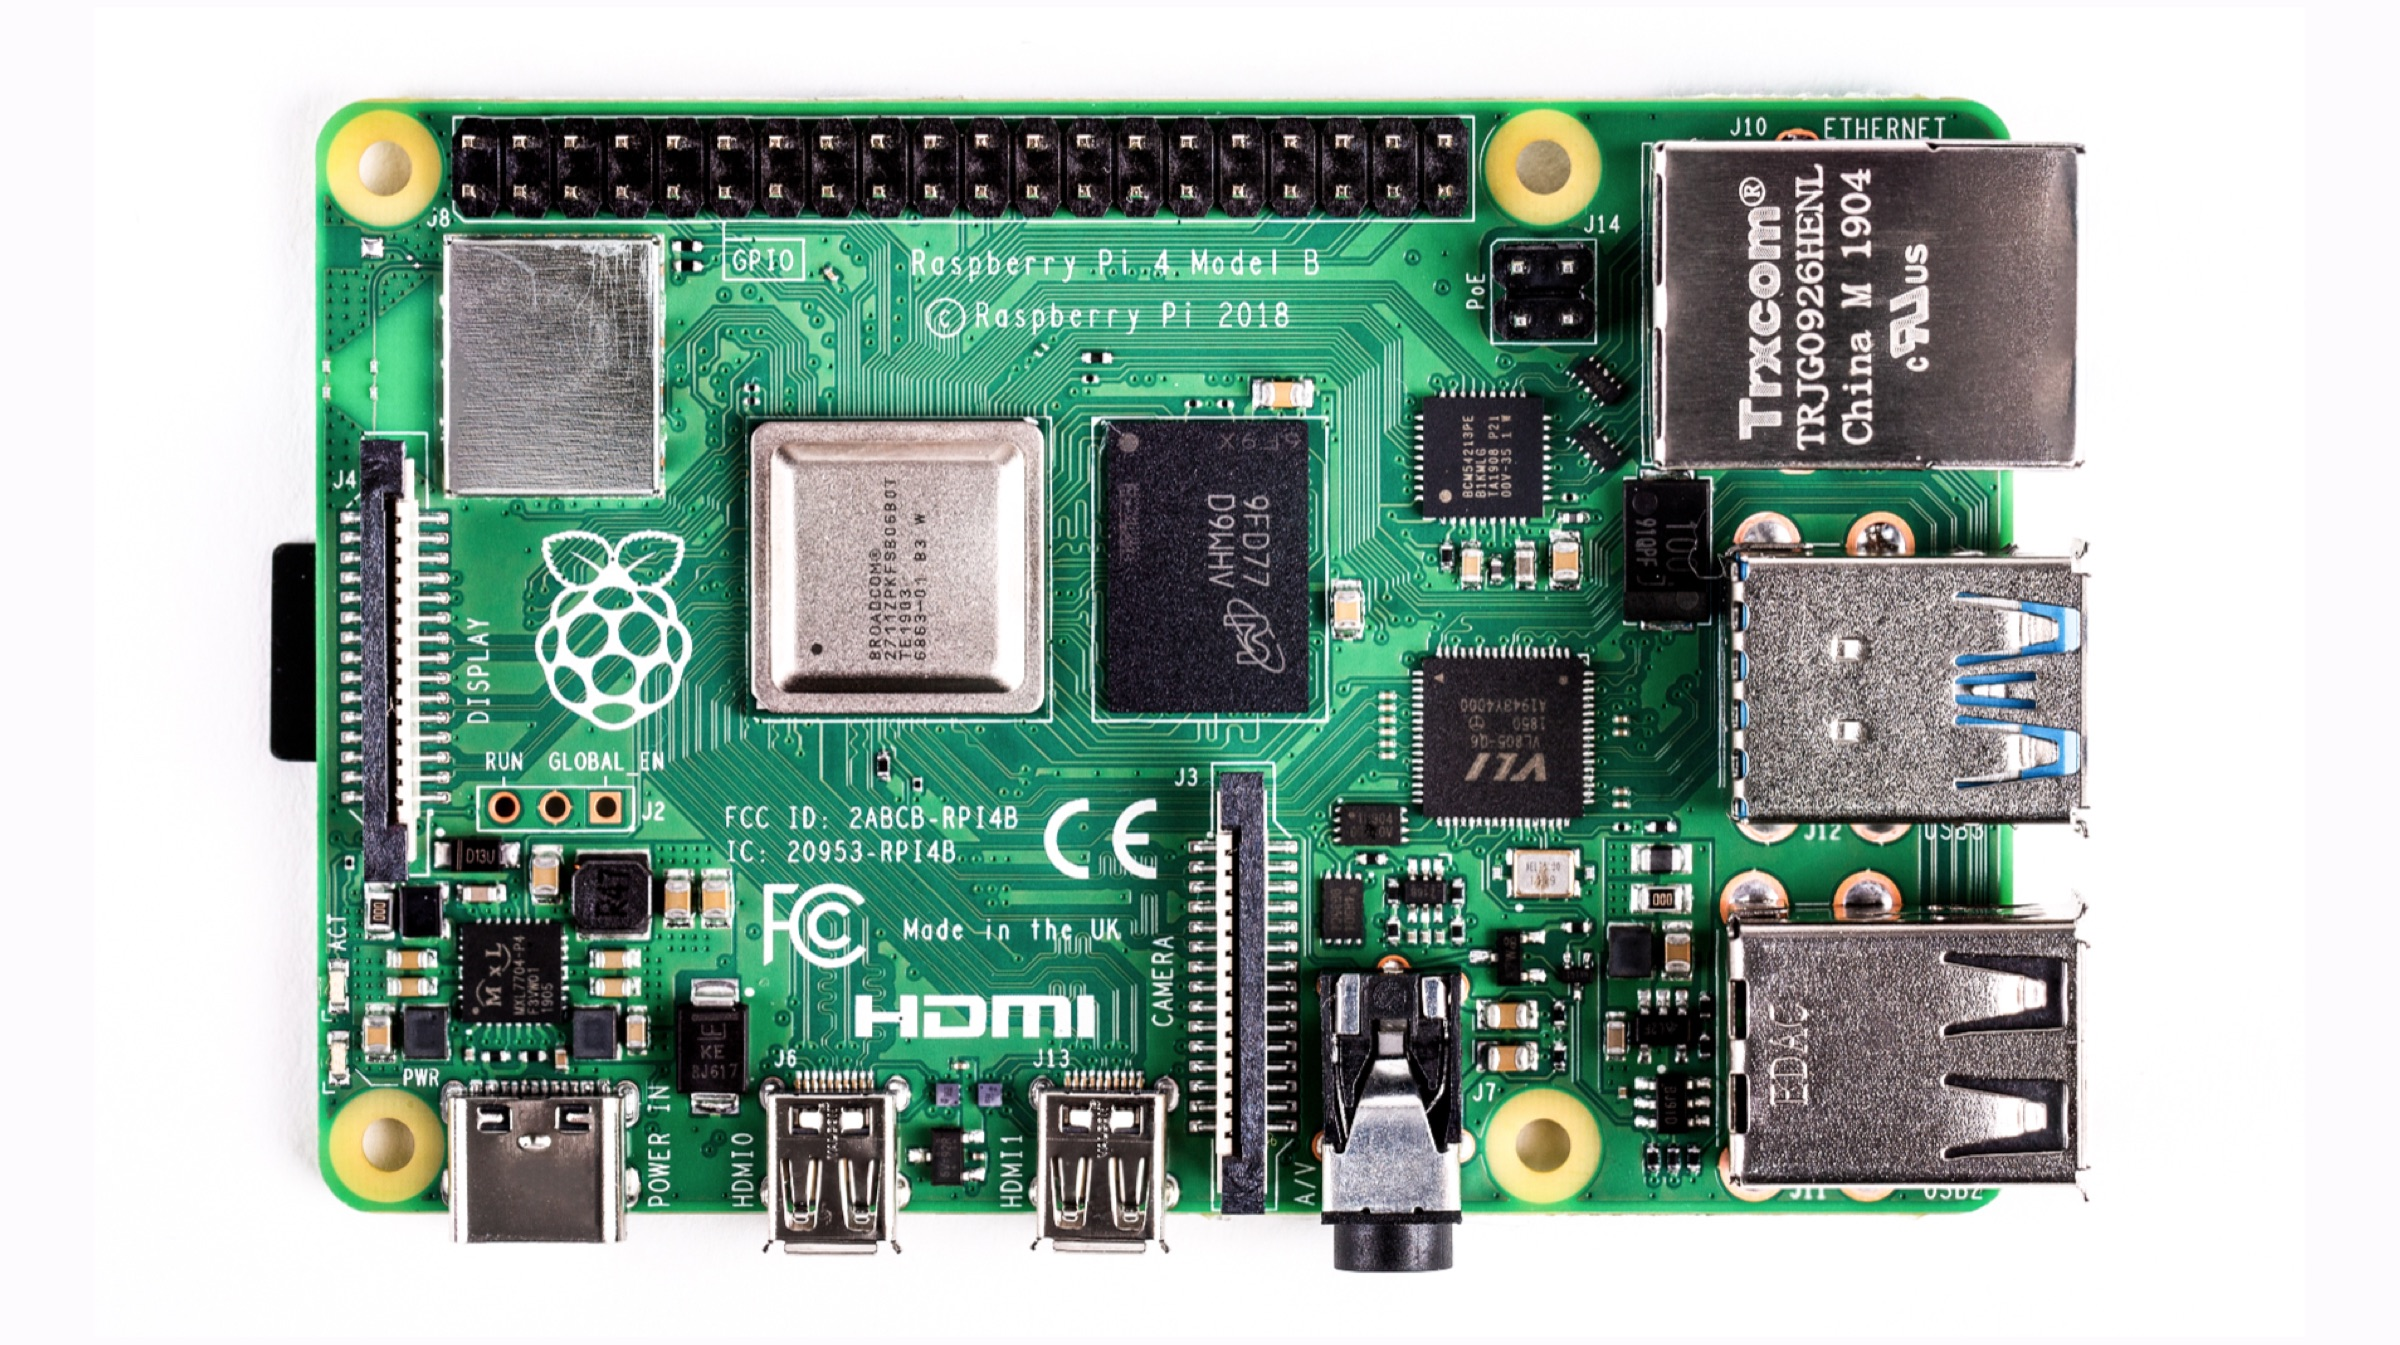
\includegraphics[width=0.6\textwidth]{../images/Raspberry-Pi-4-2}
	\caption{Raspberry Pi4}
	\label{fig:RPI4}
\end{figure}

\quad La Raspberry Pi joue un rôle clé dans l’architecture du projet 
Casiers RFID Motorisés en assurant la gestion des capteurs RFID et des actionneurs (servomoteurs et diodes RGB).

Pourquoi utiliser un Raspberry Pi ?

Le choix du Raspberry Pi 3 ou 4 repose sur plusieurs critères :

\begin{itemize}
\item Fiabilité et disponibilité : Composant largement utilisé avec un support actif.
Compatibilité : Capable de communiquer avec les lecteurs RFID et les servomoteurs via des interfaces GPIO, UART, I2C et SPI
\item Consommation énergétique faible : Adaptée aux environnements industriels avec une alimentation 5V standard
\item Facilité de développement : Compatible avec Linux (Raspberry Pi OS) et plusieurs bibliothèques de gestion de capteurs
\end{itemize}

Le Raspberry Pi est utilisé pour :

\begin{itemize}
\item Lire les badges RFID grâce à un lecteur RFID EM4100 (125 kHz) connecté sur le port série
\item Commander l’ouverture des casiers en actionnant les servomoteurs intelligents HerkuleX via une liaison série
\item Gérer l’éclairage des diodes RGB (WS2812) pour indiquer le casier actif
\item Envoyer les informations au serveur SQL via le réseau Ethernet de l’usine
\end{itemize}

Le Raspberry Pi sera installé dans un boîtier de protection, fixé à proximité des casiers et relié aux autres composants via :

\begin{itemize}
\item Un réseau Ethernet pour la communication avec la base de données
\item Un bus série pour la gestion des servomoteurs et lecteurs RFID
\item Des GPIOs pour le contrôle des diodes RGB
\end{itemize}

Ce microcontrôleur représente une solution compacte, performante et évolutive, adaptée aux besoins du projet.

\textbf{Spécifications techniques de la Raspberry PI :}

\begin{table}[h!]
\centering
\begin{tabular}{|l|l|}
\hline
\textbf{Composants} & \textbf{Détails} \\
\hline
Modèle & Raspberry Pi 4 \\
\hline
Processeur & Quad-Core ARM Cortex-A72 \\
\hline
Mémoire RAM & 2 GO \\
\hline
Stockage & Carte microSD 16GO \\
\hline
Connectivité & Ethernet \\
\hline
Interfaces & UART, GPIO, I2C, SPI, USB \\
\hline
Alimentation & 5V \\
\hline
Système d’exploitation & Debian \\
\hline
\end{tabular}
\caption{Caractéristiques techniques du Raspberry Pi 4}
\end{table}


\subsubsection{Base de données}

\begin{figure}[H]
	\centering
	
\includegraphics[width=0.6\textwidth]{../images/MariaDB}
	\caption{Logo MariaDB}
	\label{fig:MDB}
\end{figure}

\quad Dans le cadre du projet Casiers RFID Motorisés, une base de données SQL est utilisée pour stocker les identifiants des badges RFID, les associations badge/casier, ainsi que l’historique des accès. Nous avons opté pour MariaDB, une version libre et compatible de MySQL, installée sur la Raspberry Pi, puis migrée sur un serveur NUC dans un second temps.

\subsubsection{Lecteur RFID}

\begin{figure}[H]
	\centering
	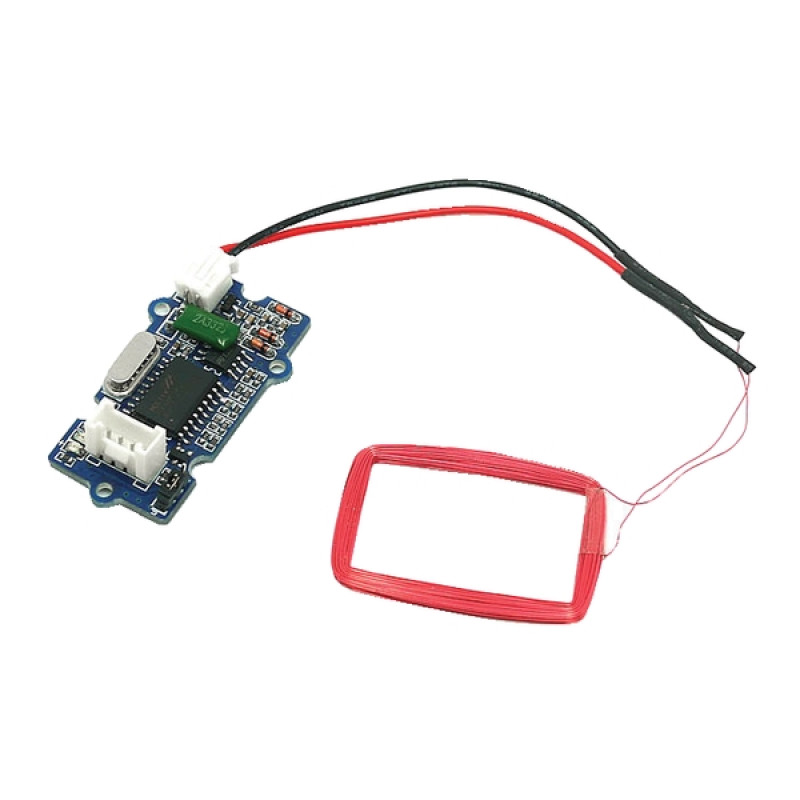
\includegraphics[width=0.7\textwidth]{../images/33140}
	\caption{Lecteur RFID UEM4100}
	\label{fig:L_RFID}
\end{figure}

\quad Le lecteur RFID est un élément central du projet Casiers RFID Motorisés, permettant l’identification des chauffeurs grâce à un badge unique. Ce système assure la correspondance entre le badge RFID et le casier attribué, facilitant ainsi la restitution automatique des documents d’identité.

Le projet utilise des lecteurs RFID UEM4100 (125 kHz) pour plusieurs raisons :

\begin{itemize}
\item Compatibilité avec les badges existants utilisés dans l’entreprise Sylvamo S.A.R.L
\item Lecture sans contact facilitant grandement l’automatisation du système
\item Fiabilité et rapidité de lecture, essentielles pour un fonctionnement fluide
\item Communication en série (UART ou USB), permettant une intégration simple avec le Raspberry Pi et l’application de gestion
\end{itemize}

Le lecteur RFID fonctionne sous une tension de 5 volts, alors que le port USB de la raspberry pi délivre seulement du 3.3 volts. Une conversion est alors nécessaire pour éviter d’endommager la raspberry pi . Cela est fait via un module de conversion 3.3 volts à 5 volts placé entre le port USB de la raspberry et le lecteur RFID.

\textbf{Deux types de lecteurs RFID sont utilisés :}

\begin{enumerate}
\item Lecteur RFID USB (poste de garde)
\begin{itemize}
\item Connecté à l’ordinateur sous Windows
\item Permet d’enregistrer un badge RFID dans la base de données lors de l’entrée d’un chauffeur
\item Associe le badge à un casier spécifique via l’application Windows
\end{itemize}
\item Lecteur RFID Série (UART) (borne de restitution)
\begin{itemize}
\item Intégré au système des casiers et connecté au Raspberry Pi
\item Lit le badge RFID lors de la restitution du chauffeur
\item Envoie l’information au Raspberry Pi, qui déclenche l’ouverture du casier correspondant
\end{itemize}
\end{enumerate}

\textbf{Intégration dans le système}

\begin{itemize}
\item À l’entrée du site, l’agent de sécurité scanne le badge RFID avec le lecteur USB pour l’enregistrer dans la base de données et l’associer à un casier
\item À la sortie, le chauffeur insère son badge RFID dans le lecteur série (UART)
\item Le Raspberry Pi analyse l’ID du badge et déclenche l’ouverture du casier attribué
\item Une diode RGB s’allume pour indiquer quel casier récupérer
\end{itemize}

Grâce à cette technologie, l’automatisation du processus de restitution est rapide, fiable et réduit les temps d’attente pour les chauffeurs.

\textbf{Spécificités techniques du lecteur RFID :}

\begin{table}[h!]
\centering
\begin{tabular}{|l|l|}
\hline
\textbf{Caractéristiques} & \textbf{Valeurs} \\
\hline
Modèle & UEM4100 \\
\hline
Fréquence & 125 kilohertz \\
\hline
Portée de lecture & 2 à 10 centimètres \\
\hline
Interface & USB (PC) / UART (SBC) \\
\hline
Alimentation & 5V \\
\hline
Protocole de communication & Série (9600 bauds) \\
\hline
\end{tabular}
\caption{Caractéristiques techniques du lecteur RFID UEM4100}
\end{table}

\subsubsection{Servomoteurs}

\begin{figure}[H]
	\centering
	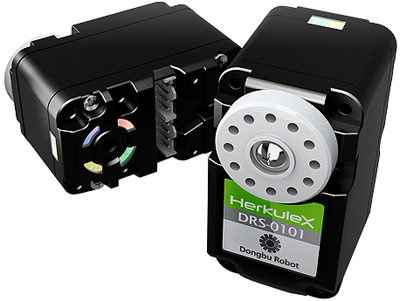
\includegraphics[width=0.7\textwidth]{../images/Servo}
	\caption{Servomoteurs Dongbu HerkuleX DRS0101}
	\label{fig:S_DH}
\end{figure}

\quad Les servomoteurs sont un élément clé du projet Casiers RFID Motorisés, assurant l’ouverture et la fermeture automatique des casiers en fonction de l’identification RFID du chauffeur.

Le projet utilise des servomoteurs intelligents Dongbu HerkuleX DRS0101, sélectionnés pour leurs caractéristiques adaptées aux besoins du système :

\begin{itemize}
\item Communication en série permettant de connecter plusieurs servomoteurs sur un même bus
\item Précision et contrôle avancé grâce à un retour d’information (position, température, état)
\item Compact et robuste, idéal pour une intégration dans un casier sécurisé
\item Faible consommation énergétique, fonctionnant en 7.4V
\end{itemize}

Chaque casier est équipé d’un servomoteur qui :

\begin{itemize}
\item Reste verrouillé tant que le badge RFID du chauffeur n’a pas été détecté
\item S’active automatiquement lorsque le badge RFID est scanné à la sortie, ouvrant ainsi le casier attribué
\item Se referme après récupération (hypothétique) du document d’identité
\end{itemize}

Un indicateur LED RGB accompagne l’ouverture pour aider visuellement le chauffeur à repérer son casier.

Intégration des servomoteurs dans le système :

\begin{itemize}
\item Le Raspberry Pi contrôle les servomoteurs via une liaison série (UART).
\item Chaque servomoteur est connecté en chaîne pour limiter le câblage et simplifier l’intégration.
\item Les commandes sont envoyées en fonction de l’identification RFID pour déclencher l’ouverture du casier approprié.
\end{itemize}

Grâce à ces servomoteurs intelligents, l’automatisation du système est fluide, rapide et fiable, tout en garantissant un faible encombrement et une consommation optimisée.

\textbf{Spécificités techniques des servomoteurs :}

\begin{table}[h!]
\centering
\begin{tabular}{|l|l|}
\hline
\textbf{Caractéristiques} & \textbf{Valeurs} \\
\hline
Modèle & Dongbu HerkuleX DRS-0101 \\
\hline
Tension d’alimentation & 7.4V \\
\hline
Couple max & 1.2nM \\
\hline
Interface & UART série (protocole TTL) \\
\hline
Angle de rotation & 320 \\
\hline
\end{tabular}
\caption{Caractéristiques techniques du servomoteur HerkuleX DRS-0101}
\end{table}

\subsection{Nuc}

\begin{figure}[H]
	\centering
	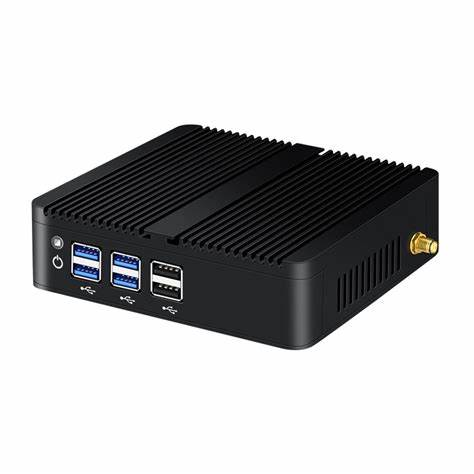
\includegraphics[width=0.6\textwidth]{../images/NUC}
	\caption{Next Unit of Computing}
	\label{fig:NUC}
\end{figure}

\quad Le NUC (Next Unit of Computing) est un mini-PC utilisé dans le projet Casiers RFID Motorisés pour héberger et gérer la base de données, tout en assurant la gestion réseau et la sécurité du système, il va jouer le rôle du pare-feu.

Le choix d’un NUC repose sur plusieurs critères :

\begin{itemize}
\item Taille compacte, facilitant l’intégration dans l’environnement industriel de l’usine
\item Consommation énergétique réduite, adaptée à une utilisation continue
\item Puissance de calcul suffisante pour exécuter une base de données et des services réseau
\item Fiabilité et évolutivité, permettant une maintenance simplifiée
\end{itemize}

Rôles du NUC dans le projet :

\begin{enumerate}
\item Hébergement de la base de données
\begin{itemize}
\item Le NUC exécute une machine virtuelle sous Proxmox, sur laquelle est installée une base de données SQL (MariaDB ou MySQL)
\item Il stocke les informations des badges RFID et des casiers associés
\end{itemize}
\item Gestion du réseau et de la sécurité
\begin{itemize}
\item Configuration du pare-feu logiciel IPFire pour sécuriser les communications entre les composants du système
\item Attribution des adresses IP fixes aux différents éléments connectés (Raspberry Pi, poste de garde, autres…)
\end{itemize}
\item Supervision et administration
\begin{itemize}
\item Permet l’accès à l’interface de gestion et de surveillance du système
\item Facilité de maintenance et mises à jour grâce à l’architecture x86 et la compatibilité avec de nombreux logiciels
\end{itemize}
\end{enumerate}

Intégration du NUC dans le système :

\begin{itemize}
\item Connexion au réseau Ethernet de l’usine pour assurer la communication avec les autres composants
\item Installation dans un espace sécurisé pour éviter tout accès non autorisé
\item Accès distant via SSH pour l’administration et la maintenance
\end{itemize}

Grâce à l’utilisation d’un NUC, le projet bénéficie d’un serveur fiable, compact et performant, garantissant un traitement rapide des données et une gestion optimisée des ressources du système.

\textbf{Spécificités techniques du NUC :}

\begin{table}[h!]
\centering
\begin{tabular}{|l|l|}
\hline
\textbf{Caractéristiques} & \textbf{Valeurs} \\ \hline
Modèle & XCY-Mini PC \\ \hline
Processeur & Intel Celeron \\ \hline
Mémoire RAM & 8 GO \\ \hline
Stockage & SSD 128GB \\ \hline
Interfaces réseau & Ethernet \\ \hline
LAN & 4 ports Ethernet \\ \hline
Système d'exploitation & Debian ipfire \\ \hline
Consommation & Faible \\ \hline
\end{tabular}
\caption{Caractéristiques techniques du NUC}
\end{table}


\newpage

\end{document}